\begin{frame}{What is ITensor?}

\begin{columns}

  \begin{column}[T]{0.7\textwidth}%

    \begin{itemize}[<+->]

      \item Stands for ``Intelligent Tensor''.
      \item Started by \textbf{Steve White} of UCI (inventor of the DMRG algorithm).
      \item Development taken over by \textbf{Miles Stoudenmire} (CCQ) around 2011.
      \item I took over development in 2018, still co-developed with Miles.
      \item Originally written in C++. I led the port to Julia starting in 2019.
      \item \textbf{Katie Hyatt} (AWS) wrote the GPU backend in Julia.
      \item Website: \myhref{https://www.itensor.org/}{itensor.org}.
      \item Paper: \myhref{https://arxiv.org/abs/2007.14822/}{arxiv.org/abs/2007.14822}.

    \end{itemize}

  \end{column}

  \begin{column}[T]{0.3\textwidth}%

    \begin{figure}[T]
      
\includegraphics[width=1.0\textwidth]{
        slides/assets/what-is-itensor-itensor.jpg
      }
    \end{figure}

    \begin{columns}

      \begin{column}[T]{0.5\textwidth}%

        \begin{figure}[T]
          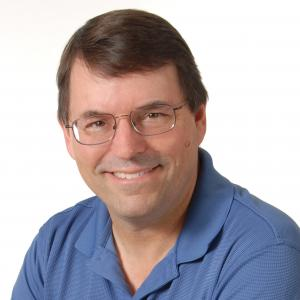
\includegraphics[width=1.0\textwidth]{
            slides/assets/what-is-itensor-steve-white.jpg
          }
        \end{figure}

        \begin{figure}[T]
          
\includegraphics[width=1.0\textwidth]{
            slides/assets/what-is-itensor-cpp.jpg
          }
        \end{figure}

      \end{column}

      \begin{column}[T]{0.5\textwidth}%

        \begin{figure}[T]
          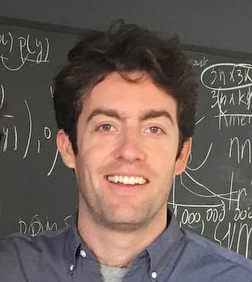
\includegraphics[width=1.0\textwidth]{
            slides/assets/what-is-itensor-miles-stoudenmire.jpg
          }
        \end{figure}

        \begin{figure}[T]
          
\includegraphics[width=1.0\textwidth]{
            slides/assets/what-is-itensor-julia.jpg
          }
        \end{figure}

      \end{column}

    \end{columns}

  \end{column}

\end{columns}

\end{frame}
